\chapter{Implementación numérica y análisis de la retroproyección filtrada}
\chaptermark{Implementación numérica y análisis de FBP}

En el capítulo anterior se estableció la fórmula continua de inversión por retroproyección filtrada y se fijó la convención
\[
f=\mathcal R^*\mathcal F_t^{-1}\bigl[|\sigma|\,\mathcal F_t(\mathcal Rf)\bigr].
\]
El objetivo de este capítulo es trasladar esa formulación a una implementación discreta reproducible, manteniendo la rampa canónica $\tau_{\mathrm{rampa}}(\sigma)=|\sigma|$ y evitando factores empíricos o normalizaciones ajustadas al fantoma.

El análisis se organiza alrededor de tres elementos: la discretización del modelo tomográfico, la aplicación de multiplicadores discretos en la variable del detector y la comparación de la rampa con seis filtros exploratorios. Los experimentos se realizan con un fantoma geométrico propio, una grilla espacial de tamaño $N=256$ y $M=90$ ángulos equiespaciados en $[0,\pi)$.

La discusión cuantitativa se apoya en métricas calculadas sobre el disco de soporte del fantoma. Los resultados no buscan identificar filtros óptimos, sino documentar cómo distintas elecciones del símbolo modifican el compromiso entre resolución y estabilidad frente al ruido bajo una configuración numérica fija.

\section{Discretización del modelo tomográfico}

La implementación numérica parte del modelo continuo descrito en los capítulos anteriores, pero reemplaza las funciones por arreglos finitos y las integrales por operaciones discretas. En esta sección se fijan las grillas espaciales, angulares y de detector usadas en todos los experimentos del capítulo.

\subsection*{Discretización del dominio espacial}

Se considera una malla cartesiana uniforme semiabierta en $[-1,1)^2$ de tamaño $N\times N$, con $N=256$. Con paso espacial $h=2/N$, los nodos se escriben como
\[
x_i=\left(i-\frac{N}{2}\right)h,\qquad
y_j=\left(j-\frac{N}{2}\right)h,
\qquad i,j=0,\ldots,N-1.
\]
Así, el índice $N/2=128$ representa exactamente el origen. Esta elección coincide con la convención de \texttt{scikit-image} 0.26.0, que sitúa el eje de rotación de \texttt{radon} en el píxel de índices \texttt{(N//2,N//2)} \cite{scikitimage_radon026}.
El fantoma utilizado es geométrico, asimétrico y está contenido en el disco
\[
x^2+y^2\le R^2,
\qquad R=0.9.
\]
No se usa el fantoma de Shepp--Logan como caso principal, porque se busca un objeto sintético simple con inclusiones de distintas intensidades y posiciones no simétricas.

\subsection*{Grilla angular y detector}

Los ángulos se toman uniformemente en $[0,\pi)$ mediante
\[
\theta_k=k\Delta\theta,
\qquad k=0,\ldots,M-1,
\]
con
\[
M=90,
\qquad \Delta\theta=2^\circ=\frac{\pi}{90}.
\]
Para cada ángulo se genera una proyección discreta, y el conjunto de proyecciones forma un sinograma
\[
g\in\mathbb R^{N_t\times M},
\qquad N_t=256.
\]
La variable del detector se discretiza como
\[
t_\ell=(\ell-N_t/2)\Delta t,
\qquad \ell=0,\ldots,N_t-1,
\]
donde $\Delta t=h=2/N$. El índice $N_t/2=128$ corresponde exactamente a $t=0$ y coincide con el eje del sinograma, que la implementación ubica en \texttt{N\_t//2} \cite{scikitimage_radon026}.

\subsection*{Generación del sinograma}

El sinograma se genera con la rutina \texttt{radon} de \texttt{scikit-image} \cite{vanderwalt2014scikitimage}, usando la opción \texttt{circle=True}. En la versión 0.26.0, esta opción supone que la imagen es nula fuera del círculo inscrito en la malla y hace que el ancho de cada proyección sea igual a la menor dimensión de la imagen \cite{scikitimage_radon026}; por ello se conserva $N_t=N=256$. No describe una geometría de adquisición circular: la adquisición sigue correspondiendo a una geometría de haz paralelo.\\

La definición geométrica continua no se modifica: la recta asociada a $(t,\theta)$ sigue dada por $x\cdot\omega(\theta)=t$, con $\omega(\theta)=(\cos\theta,\sin\theta)$. La implementación debe, sin embargo, distinguir esta convención matemática de la orientación vertical de las matrices digitales, cuyas filas crecen en sentido opuesto al eje cartesiano usual. Esta diferencia se corrige al retroproyectar, sin cambiar la definición de la transformada de Radon.\\

La Figura~\ref{fig:chapter3-phantom-sinogram} muestra el fantoma y el sinograma generado con estos parámetros.

\begin{figure}[htbp]
    \centering
    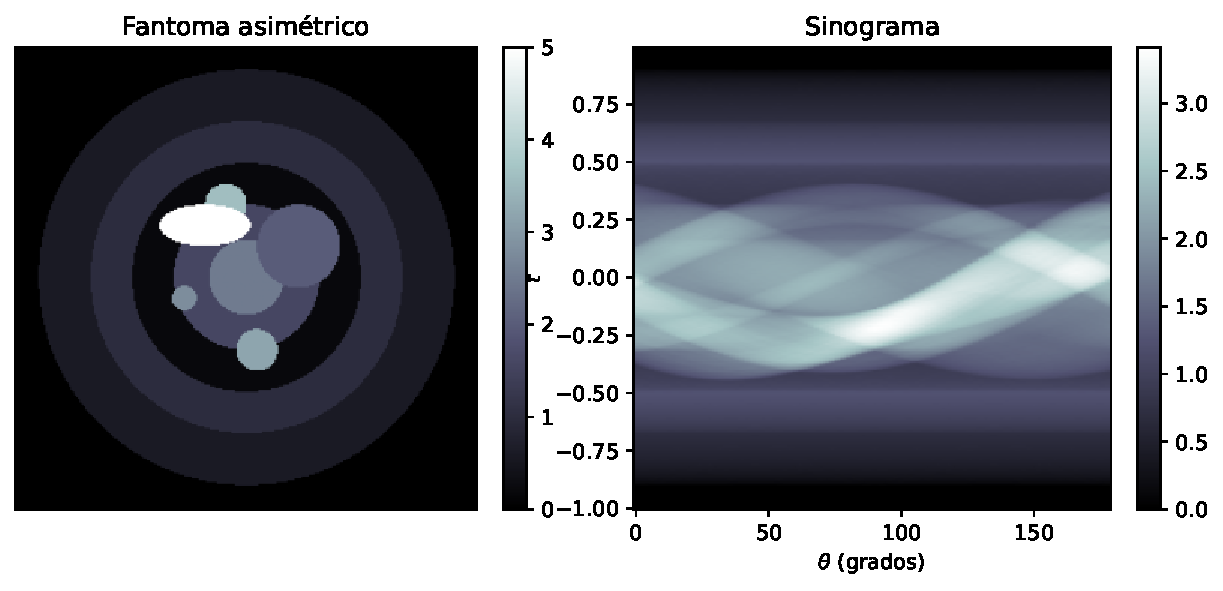
\includegraphics[width=0.92\textwidth]{Figures/Chapter3/phantom_and_sinogram.pdf}
    \caption{Fantoma geométrico utilizado en los experimentos y sinograma generado con $M=90$ ángulos de haz paralelo. El fantoma está contenido en el disco de radio $R=0.9$, y el sinograma constituye el dato de entrada para las reconstrucciones posteriores.}
    \label{fig:chapter3-phantom-sinogram}
\end{figure}

Esta discretización es suficiente para estudiar el comportamiento relativo de los filtros considerados. Existen formulaciones formales de transformadas de Radon discretas, como la de Beylkin \cite{beylkin1987}, pero la implementación de esta tesis corresponde a un modelo muestreado basado en sinogramas generados numéricamente y no a una implementación exacta de dicha transformada discreta. Los errores introducidos por interpolación, muestreo espacial y muestreo angular forman parte del modelo numérico evaluado y no se corrigen mediante ajustes posteriores de amplitud \cite{kak_slaney1988,natterer2001}.

\section{Algoritmo discreto de retroproyección filtrada}

La retroproyección filtrada discreta implementa la fórmula continua de FBP mediante operaciones finitas en la variable del detector y una cuadratura angular. En esta sección se separan la retroproyección sin filtrar, el filtrado por columnas y la reconstrucción final.

\subsection*{Retroproyección discreta}

El operador continuo de retroproyección está dado por
\[
\mathcal R^*g(x)=\int_0^\pi g(x\cdot\omega(\theta),\theta)\,d\theta,
\]
con $\omega(\theta)=(\cos\theta,\sin\theta)$. En la malla discreta se aproxima por
\[
(\mathcal R_d^*g)_{i,j}
=
\Delta\theta\sum_{k=0}^{M-1}
\mathcal I_t\bigl[g_{\cdot,k}\bigr]
\bigl(t(x_i,y_j,\theta_k)\bigr),
\]
donde $\mathcal I_t$ denota interpolación lineal en la variable del detector. La geometría matemática usa $t(x,y,\theta)=x\cdot\omega(\theta)$; en la implementación matricial se toma en cuenta la orientación vertical de las filas para evaluar correctamente las coordenadas cartesianas.

La retroproyección sin filtrar se obtiene aplicando directamente este operador al sinograma:
\[
f_{\mathrm{BP}}=\mathcal R_d^*g.
\]
Como se discutió en el capítulo anterior, $\mathcal R^*\mathcal R$ no es la identidad; por ello esta reconstrucción presenta difuminado y requiere filtrado previo.

\subsection*{Filtrado discreto por columnas}

El filtrado se aplica independientemente a cada columna angular $g_{\cdot,k}\in\mathbb R^{N_t}$. Para distinguir la transformada de Fourier continua de la transformada discreta usada en el código, se introducen los siguientes operadores:
\begin{itemize}
    \item $P:\mathbb R^{N_t}\to\mathbb R^{N_{\mathrm{fft}}}$, operador de zero-padding centrado.
    \item $C:\mathbb R^{N_{\mathrm{fft}}}\to\mathbb R^{N_t}$, operador de recorte al intervalo detector original.
    \item $F_{N_{\mathrm{fft}}}$, DFT de longitud $N_{\mathrm{fft}}$.
    \item $M_\tau[m]=\tau(\sigma_m)$, vector multiplicador evaluado en la grilla de frecuencias $\sigma_m$ generada con \texttt{fftfreq}.
\end{itemize}

Para cada columna angular se calcula
\[
g^\tau_{\cdot,k}
=
C F_{N_{\mathrm{fft}}}^{-1}
\operatorname{diag}(M_\tau)
F_{N_{\mathrm{fft}}}
P g_{\cdot,k}.
\]
En los experimentos se usa
\[
N_t=256,
\qquad
N_{\mathrm{fft}}=1024.
\]
La longitud $N_{\mathrm{fft}}$ es auxiliar: no añade datos ni resolución espacial. Su función es reducir los efectos de tratar directamente cada proyección finita como si fuera periódica, es decir, mitigar artefactos asociados a la convolución circular de la DFT.

\subsection*{Reconstrucción filtrada}

Luego de filtrar todas las columnas, la reconstrucción se define como
\[
f_\tau=\mathcal R_d^*g^\tau.
\]
Para la rampa canónica,
\[
\tau_{\mathrm{rampa}}(\sigma)=|\sigma|,
\]
esta expresión es la contraparte discreta de
\[
f=\mathcal R^*\mathcal F_t^{-1}\bigl[|\sigma|\,\mathcal F_t(\mathcal Rf)\bigr].
\]
No se introducen factores $1/2$, $1/\pi$, correcciones empíricas ni reescalamientos de las reconstrucciones.

La Figura~\ref{fig:chapter3-bp-vs-fbp} compara la retroproyección sin filtrar con la reconstrucción FBP usando la rampa.

\begin{figure}[htbp]
    \centering
    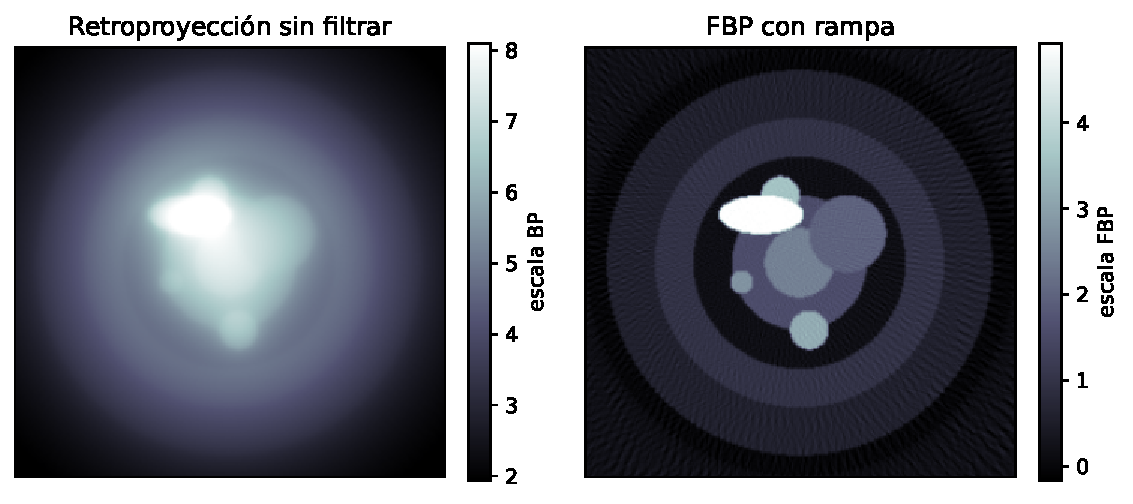
\includegraphics[width=0.86\textwidth]{Figures/Chapter3/bp_vs_fbp.pdf}
    \caption{Comparación entre la retroproyección sin filtrar y la retroproyección filtrada con la rampa. La retroproyección directa produce una imagen difuminada, mientras que el filtrado previo compensa parcialmente el suavizado asociado a $\mathcal R^*\mathcal R$.}
    \label{fig:chapter3-bp-vs-fbp}
\end{figure}

\section{Símbolos discretos y filtros A--F}

El algoritmo anterior queda determinado por el símbolo $\tau$ usado para construir el multiplicador discreto $M_\tau$. En esta sección se describen los siete símbolos evaluados: la rampa como referencia y seis filtros exploratorios, denotados A--F.

\subsection*{Rampa de referencia}

El símbolo de referencia es la rampa canónica
\[
\tau_{\mathrm{rampa}}(\sigma)=|\sigma|.
\]
Esta elección corresponde directamente a la fórmula continua de FBP fijada en el Capítulo 2. En la implementación discreta no se introduce ningún factor adicional en este símbolo.

\subsection*{Filtros exploratorios A, B y C}

El filtro A modifica la rampa mediante una perturbación oscilatoria dependiente de la frecuencia:
\[
\tau_A(\sigma)
=
|\sigma|\left(1+\frac{\sin|\sigma|}{1+|\sigma|}\right).
\]
El filtro B tiene respuesta no nula en frecuencia cero:
\[
\tau_B(\sigma)=\sqrt{0.3^2+|\sigma|^2}.
\]
En particular, $\tau_B(0)=0.3$. En cambio, la rampa y los filtros A, C, D, E y F se anulan en frecuencia cero.\\

El filtro C introduce un corte compacto relativo a la frecuencia máxima de la grilla discreta:
\[
\tau_C(\sigma)
=
|\sigma|\left(1-\frac{|\sigma|}{\sigma_c}\right)_+,
\qquad
\sigma_c=0.6\sigma_{\max}.
\]
Aquí $(a)_+=\max\{a,0\}$.

\subsection*{Filtros D, E y F}

Los filtros D, E y F crecen como la rampa hasta $|\sigma|=20$ y luego modifican el tratamiento de frecuencias mayores. El filtro D es triangular:
\[
\tau_D(\sigma)=
\begin{cases}
|\sigma|, & |\sigma|\le 20,\\
40-|\sigma|, & 20<|\sigma|\le 40,\\
0, & |\sigma|>40.
\end{cases}
\]
El filtro E usa decaimiento exponencial moderado:
\[
\tau_E(\sigma)=
\begin{cases}
|\sigma|, & |\sigma|\le 20,\\
20\exp[-0.08(|\sigma|-20)], & |\sigma|>20.
\end{cases}
\]
El filtro F usa decaimiento exponencial más rápido:
\[
\tau_F(\sigma)=
\begin{cases}
|\sigma|, & |\sigma|\le 20,\\
20\exp[-0.50(|\sigma|-20)], & |\sigma|>20.
\end{cases}
\]

Estos seis filtros no se presentan como filtros óptimos. Su propósito es explorar, bajo una misma configuración numérica, cómo distintas respuestas espectrales alteran la reconstrucción y su sensibilidad al ruido. Esta pregunta se relaciona con el análisis de error y el diseño de funciones filtro en FBP \cite{beckmann_iske2017,beckmann_nickel2025}, pero los símbolos A--F usados aquí no se derivan de esos trabajos ni reproducen sus filtros optimizados.

La Figura~\ref{fig:chapter3-symbols} muestra la rampa y los filtros A--F sobre la grilla de frecuencias usada por la DFT.

\begin{figure}[htbp]
    \centering
    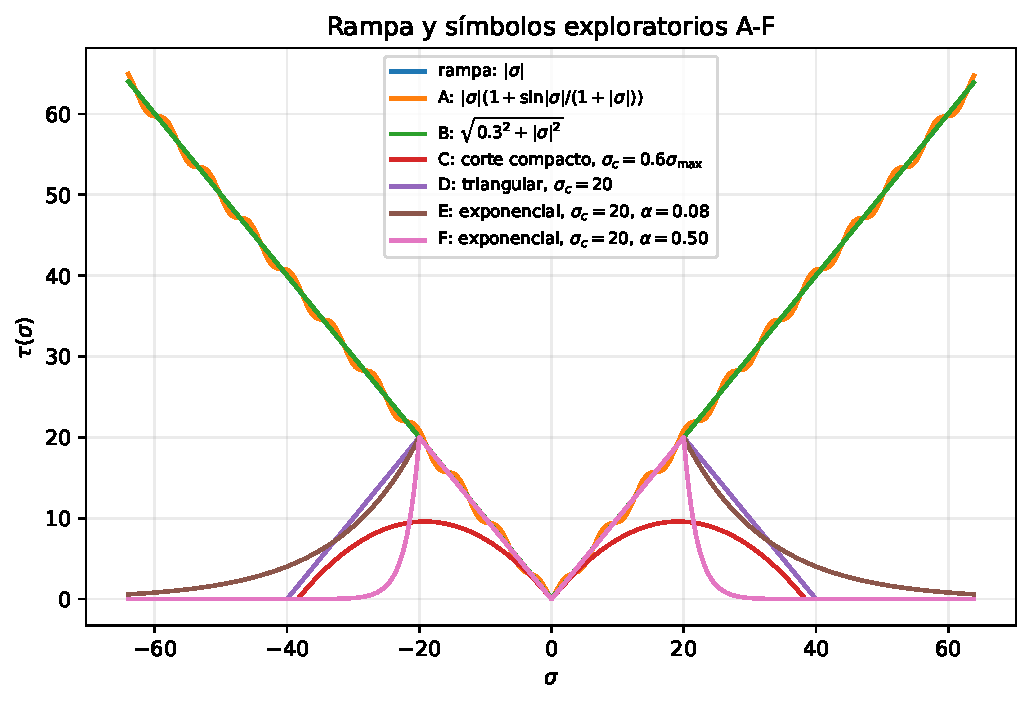
\includegraphics[width=0.86\textwidth]{Figures/Chapter3/symbols_ramp_A_F.pdf}
    \caption{Símbolos discretos evaluados sobre la grilla de frecuencias de longitud $N_{\mathrm{fft}}=1024$. La rampa se usa como referencia; los símbolos A--F son filtros exploratorios para estudiar el efecto de distintas modificaciones espectrales.}
    \label{fig:chapter3-symbols}
\end{figure}

\section{Diseño experimental y reproducibilidad}

Los experimentos del capítulo se generan de forma reproducible a partir del código incorporado en el repositorio. Esta sección resume los parámetros, el modelo de ruido, las métricas y las verificaciones automáticas usadas para producir las figuras y tablas.

\subsection*{Parámetros canónicos}

La configuración numérica es fija en todos los experimentos:
\[
N=256,
\qquad
R=0.9,
\qquad
N_t=256,
\qquad
N_{\mathrm{fft}}=1024,
\]
\[
M=90,
\qquad
\Delta\theta=2^\circ,
\qquad
\texttt{circle=True}.
\]
La opción \texttt{circle=True} impone la hipótesis de soporte en el círculo inscrito y mantiene $N_t=256$ muestras de detector; no modifica la geometría de adquisición de haz paralelo. La longitud $N_{\mathrm{fft}}=1024$ se usa solo como longitud auxiliar para el filtrado por FFT con zero-padding centrado.\\

El código de reproducción se ejecuta desde la raíz del repositorio mediante
\[
\texttt{python code/generate\_chapter3.py}.
\]
Las versiones de NumPy, SciPy, scikit-image y Matplotlib están fijadas en el archivo de requisitos del código. Los detalles de cada corrida se registran en los metadatos de resultados, y la auditoría de normalización queda guardada junto con esos resultados.

\subsection*{Ruido}

Para evaluar estabilidad se añade ruido gaussiano aditivo al sinograma:
\[
g_{\mathrm{ruido}}=g+\eta,
\qquad
\eta_{\ell,k}\sim\mathcal N(0,\sigma_{\mathrm{noise}}^2),
\]
con
\[
\sigma_{\mathrm{noise}}=0.05\max |g|.
\]
La semilla aleatoria es $42$, y la misma realización ruidosa se usa para todos los filtros. Por tanto, las diferencias observadas bajo ruido se deben al filtrado y no a cambios en la muestra aleatoria.

\subsection*{Métricas}

Las métricas se calculan únicamente sobre los índices correspondientes al disco de soporte del fantoma:
\[
\mathcal I_R=\{(i,j):x_i^2+y_j^2\le R^2\}.
\]
Si $u$ es el fantoma y $v$ una reconstrucción, se usa
\[
\mathrm{RMSE}(u,v)
=
\left(
\frac{1}{\#\mathcal I_R}
\sum_{(i,j)\in\mathcal I_R}
(u_{i,j}-v_{i,j})^2
\right)^{1/2},
\]
y el error relativo en norma discreta $\ell^2$,
\[
\mathrm{Err}_{\ell^2}(u,v)
=
\frac{
\left(\sum_{(i,j)\in\mathcal I_R}(u_{i,j}-v_{i,j})^2\right)^{1/2}
}{
\left(\sum_{(i,j)\in\mathcal I_R}u_{i,j}^2\right)^{1/2}
}.
\]
La tabla de resultados también reporta la razón de medias entre reconstrucción y fantoma sobre $\mathcal I_R$. Esta cantidad se conserva solo como diagnóstico de amplitud; no es una métrica principal ni se utiliza como factor de escala.

\subsection*{Verificaciones automáticas}

La generación comprueba dimensiones de imagen, sinograma y multiplicadores; ausencia de valores no finitos; paridad de los símbolos; valores en frecuencia cero; aplicación independiente por columnas; orientación espacial; y reproducibilidad del hash de métricas al ejecutar dos veces con la misma semilla. No se normalizan las reconstrucciones contra el fantoma ni se aplica corrección empírica de amplitud.

\section{Resultados y discusión}

Esta sección integra las reconstrucciones y métricas generadas con la configuración descrita. La interpretación se limita a los filtros evaluados, al fantoma usado y a la realización de ruido considerada.

\subsection*{Reconstrucciones sin ruido}

La Figura~\ref{fig:chapter3-recon-noiseless} muestra las reconstrucciones obtenidas a partir del sinograma sin ruido. Visualmente, la rampa recupera la estructura principal del fantoma y obtiene el menor error relativo, mientras que los filtros E y D producen resultados cercanos entre sí según las métricas de la Tabla~\ref{tab:chapter3-metrics}.

\begin{figure}[htbp]
    \centering
    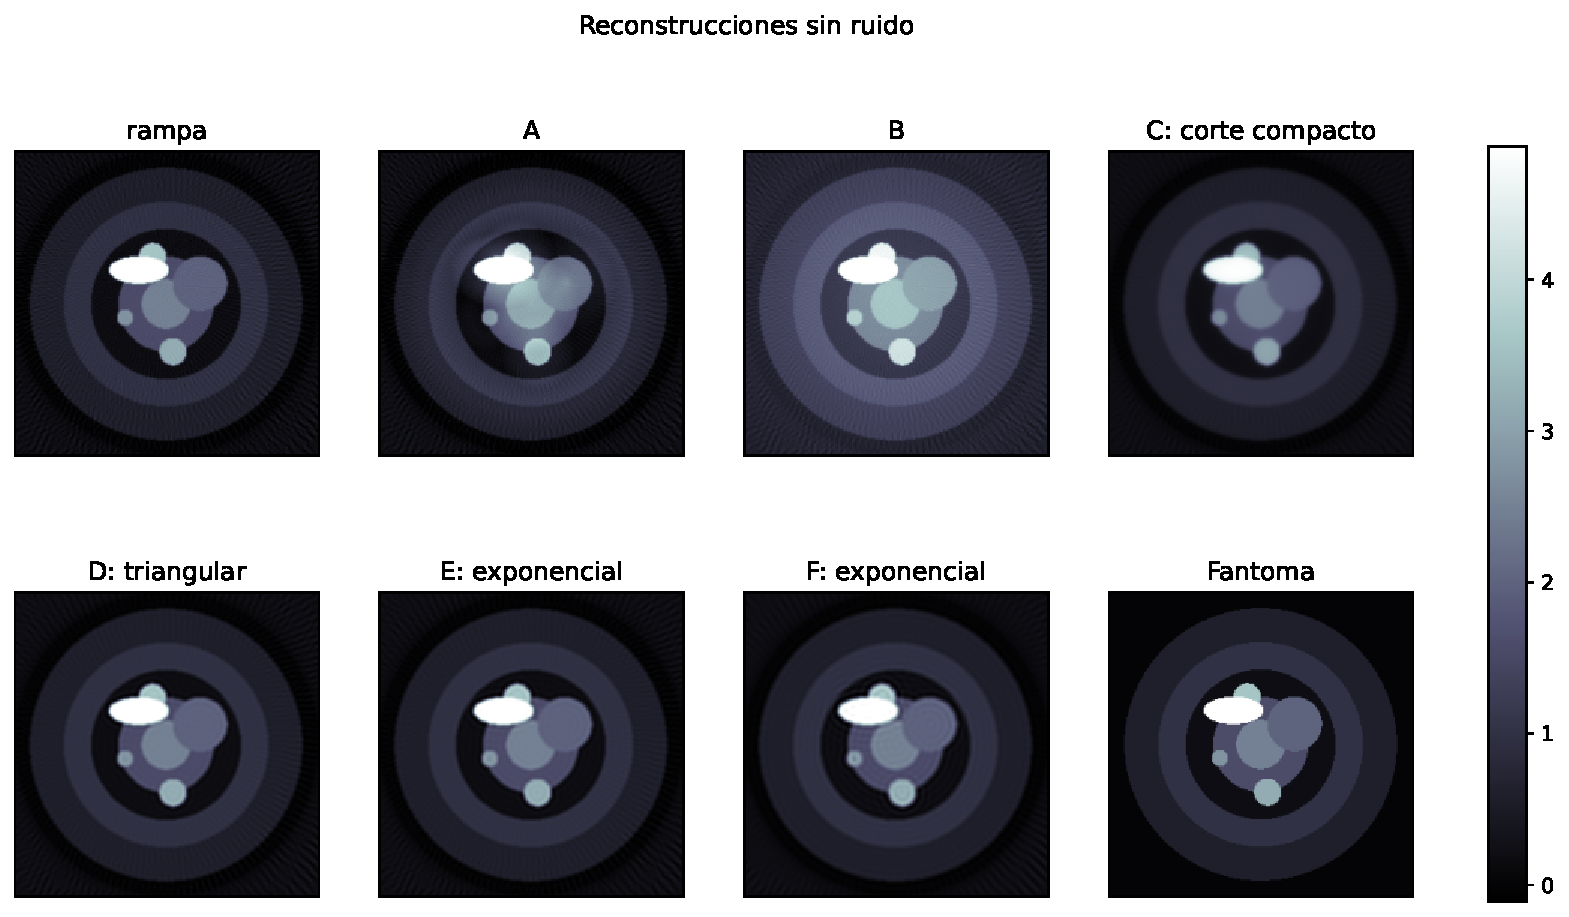
\includegraphics[width=0.96\textwidth]{Figures/Chapter3/reconstructions_noiseless.pdf}
    \caption{Reconstrucciones obtenidas sin ruido para la rampa y los filtros A--F. El último panel muestra el fantoma de referencia bajo la misma escala de color usada para las reconstrucciones, lo que permite comparar amplitud y estructura visual.}
    \label{fig:chapter3-recon-noiseless}
\end{figure}

En términos de error relativo, el menor valor sin ruido corresponde a la rampa, con $0.097892$. Le siguen E, con $0.112767$, y D, con $0.113110$; la diferencia entre estos dos filtros es pequeña en esta configuración. F obtiene $0.127115$ y C alcanza $0.143042$, mientras que A y B presentan errores mayores, $0.253226$ y $0.687715$, respectivamente.

\subsection*{Reconstrucciones con ruido}

La Figura~\ref{fig:chapter3-recon-noisy} muestra las reconstrucciones obtenidas a partir del sinograma perturbado con ruido gaussiano. Bajo la realización de ruido considerada, los filtros que atenúan altas frecuencias reducen de forma marcada la amplificación del ruido respecto de la rampa.

\begin{figure}[htbp]
    \centering
    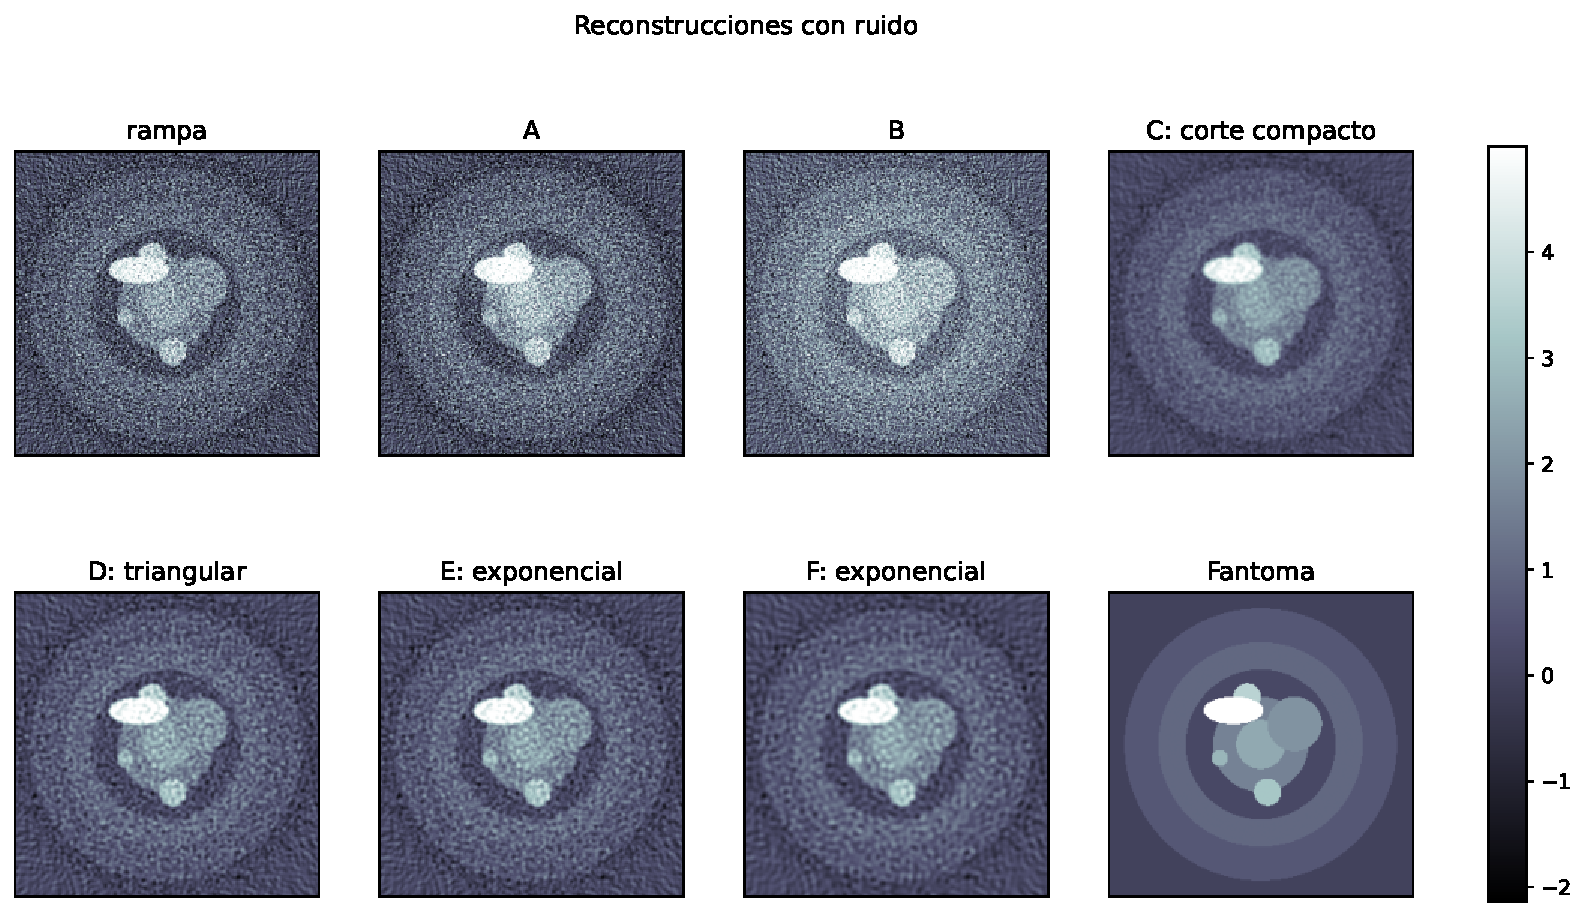
\includegraphics[width=0.96\textwidth]{Figures/Chapter3/reconstructions_noisy.pdf}
    \caption{Reconstrucciones obtenidas a partir de un único sinograma ruidoso, común a todos los filtros. Las diferencias visuales reflejan el compromiso entre preservación de detalle y atenuación de altas frecuencias bajo la realización de ruido considerada.}
    \label{fig:chapter3-recon-noisy}
\end{figure}

Entre los filtros evaluados, C obtiene el menor error relativo con ruido, $0.266386$, seguido por F con $0.318981$. Los filtros E y D quedan en un rango intermedio, con $0.383664$ y $0.390949$, respectivamente. La rampa y A presentan errores relativos mayores, $1.134227$ y $1.157932$, consistentes con una mayor amplificación de altas frecuencias. El filtro B alcanza $1.323399$; su comportamiento desfavorable es consistente con su respuesta no nula en frecuencia cero y su mayor peso de bajas frecuencias, aunque este experimento no constituye una demostración causal completa.

\subsection*{Métricas cuantitativas}

La Tabla~\ref{tab:chapter3-metrics} resume RMSE, error relativo y razón de medias. RMSE y error relativo son las métricas principales. La razón de medias se incluye únicamente como diagnóstico de amplitud y no se usa para reescalar ni para seleccionar filtros.

\begin{table}[htbp]
    \centering
    \caption{Métricas de reconstrucción calculadas sobre los índices $\mathcal I_R=\{(i,j):x_i^2+y_j^2\le R^2\}$. RMSE y error relativo en norma $\ell^2$ son las métricas principales; la razón de medias se reporta únicamente como diagnóstico de amplitud.}
    \label{tab:chapter3-metrics}
    \small
    \begin{tabular}{llrrr}
\toprule
Caso & Filtro & RMSE & Error relativo $\ell^2$ & Razón media \\
\midrule
sin ruido & rampa & 0.125294 & 0.097892 & 0.976683 \\
sin ruido & A & 0.324107 & 0.253226 & 1.181567 \\
sin ruido & B & 0.880214 & 0.687715 & 1.906510 \\
sin ruido & C: corte compacto & 0.183081 & 0.143042 & 0.963424 \\
sin ruido & D: triangular & 0.144770 & 0.113110 & 0.975620 \\
sin ruido & E: exponencial & 0.144332 & 0.112767 & 0.975596 \\
sin ruido & F: exponencial & 0.162695 & 0.127115 & 0.975090 \\
con ruido & rampa & 1.451709 & 1.134227 & 0.978050 \\
con ruido & A & 1.482050 & 1.157932 & 1.183776 \\
con ruido & B & 1.693833 & 1.323399 & 1.908387 \\
con ruido & C: corte compacto & 0.340951 & 0.266386 & 0.964867 \\
con ruido & D: triangular & 0.500380 & 0.390949 & 0.977034 \\
con ruido & E: exponencial & 0.491055 & 0.383664 & 0.977022 \\
con ruido & F: exponencial & 0.408268 & 0.318981 & 0.976554 \\
\bottomrule
\end{tabular}

\end{table}

Los resultados ilustran el compromiso entre resolución y estabilidad: sin ruido, las respuestas próximas a la rampa conservan mejor los detalles; con ruido, atenuar altas frecuencias reduce el error a costa de suavizado. El desempeño de C se limita a esta configuración y realización de ruido, sin implicar superioridad universal.

